
The participating roles in the software development process are defined in
CENELEC EN 50128~\cite{EN-50128} Figure~2 (in this document
Figure~\ref{fig:preferred-roles}). In the following all references to ``the
standard'' refer to CENELEC EN 50128:2011~\cite{EN-50128}.

We will first list and describe the roles in
Section~\ref{sec:participating-roles}, then we will shortly describe the SW
planning phase in Section~\ref{sec:documents--plan} and present the overall
lifecycle phases in Section~\ref{sec:lifecycle-phases}. A detailed description
for the system development phase is given in Section~\ref{sec:syst-devel-phase}
and for each of the SW development phases in
Section~\ref{sec:sw-development-phase}. Section~\ref{sec:conclusion-fm-process}
gives a short conclusion on the proposed development process for openETCS.

\subsection{Participating Roles}
\label{sec:participating-roles}

Each of the participants must be noted and his name and role recorded. Which
role can be taken by the same person is regulated as shown in
Figure~\ref{fig:preferred-roles}.

\subsubsection{Requirements Manager (RQM)}
\label{sec:requ-magang-rqm}

The main task of the RQM is to take care of the software requirements. He shall
specify the software requirements, ensure the traceability between them and the
system level requirements and ensure the consistency of the SW requirement
specification.

\subsubsection{Designer (DES)}
\label{sec:designer}

The main task of the DES is to create acceptable solutions from the SW
requirement specifications. He is responsible for the decisions which design
methods to apply and which tools to use. The DES develops the software component
specifications and ensures the traceability and consistency of these
specifications and the SW requirements specification.

\subsubsection{Implementer (IMP)}
\label{sec:implementer}

The main task of the IMP is the transformation of the software design solution
into source code, domain specific languages (DSL) or other appropriate
formalisms. Besides the implementation he shall produce the documentation
describing the implementation, the applied methods, data types and data
structures. He shall also ensure the traceability between the implementation and
the SW design. The IMP shall apply the specified coding standards, use the
specified programming languages and the safety design principles.

\subsubsection{Tester (TST)}
\label{sec:tester}

The TST ensures that all test activities are planned and shall produce the test
specification which includes the test cases and their objectives. He is
responsible to assure the execution of the SW tests, the recording of their
outcomes and to select the test equipments and methods. The TST shall identify
deviations from the specifications in the report and communicate them to the
change management.

\subsubsection{Verifier (VER)}
\label{sec:verifier}

The VER is responsible to produce the SW verification plan which specifies what
and how it has to be verified and what has to be produced as evidence. He shall
identify and evaluate all anomalies according to their potential impact and risk
and communicate all deviations to the change management body for further
evaluation and decision. The VER records all outcomes of the verification
activities and shall produce the verification report. The VER shall manage the
verification process and ensure the required independence of the activities.

\subsubsection{Integrator (INT)}
\label{sec:integrator}

The INT shall manage the test of the integration of the developed SW and of the
integration of the SW into the target HW based on the design specification. He
shall specify the necessary integration sequence, the necessary input components
and the expected resulting components. The INT shall record any anomalies and
deviations from the integration test specification, communicate them the change
management and produce a system integration report of the overall outcome.

\subsubsection{Validator (VAL)}
\label{sec:validator}

The VAL is responsible for the creation of the validation plan. He ensures that
the software requirements meet the intended usage in the specified application
area and environment. For this he will develop an understanding of the system
and its intended environment. He shall then review the developed SW against the
SW specification, evaluate the conformity of the development process to the
standard and the assigned SIL. He shall review the correctness, consistency and
adequacy of the verification, testing, test cases and executed tests, as well as
ensuring that the validation plan was carried out completely.

Based on these analyses he will review the deviations, classify them in terms
of risk, communicate them to the change management and shall give a
recommendation on the suitability of the developed SW for the intended task, as
well as indicate necessary constraints.

He shall audit and review the overall project wrt. generic development process,
in particular verify the traceability of all SW requirements. He shall ensure
that all remaining non-conformities are resolved directly or by risk control /
transfer measures. Finally the VAL shall produce a validation report and give
his agreement or disagreement for the release of the SW. The produced documents
shall be transmitted to the assessor.

\subsubsection{Assessor (ASR)}
\label{sec:assessor}

The ASR shall develop an assessment plan which is communicated to the safety
authority and the client. The ASR will develop an understanding of the system
and its intended environment and shall evaluate the competency of the project
staff and the organization, the verification and validation with their
supporting evidence, the quality management of the development process and the
configuration and change management with its evidence of use and application.

He shall identify and evaluate the risk of the deviations from the SW
specification, produce an assessment report and ensure that the assessment plan
is executed. He shall carry out audits and inspections of the overall
development process and give a professional view on the fitness of the developed
SW for its intended use. Based on this he shall produce an assessment report and
record there his findings of the assessment process.

\subsubsection{Project Manager (PM)}
\label{sec:project-manager}

The main task of the project manager is to ensure the independence of the roles
and organizations as specified in CENELEC EN 50128. He shall be responsible to
allocate the necessary resources, ensure the competency for the allocated rules
and allow sufficient time for the proper implementation of all required
tasks. The PM shall ensure that safety requirements of other stakeholders are
met and is responsible for the delivery and deployment of the SW. He shall
endorse safety deliverables and ensure sufficient records and the traceability
of requirements for safety related decisions.

\subsubsection{Configuration Manager (CM)}
\label{sec:conf-manag}

The CM shall be responsible for the SW configuration management plan. He owns
the configuration management system and ensures the clear identification and
independent versioning of the SW components. The CM shall prepare Release Notes
for the SW and document incompatible components if applicable.

\subsection{Software Planning Phase}
\label{sec:documents--plan}

For compliance with the standard, a certain number of plans are agreed in the SW
planning phase. These plans shall be used and updated in all development
phases. The PM shall decide the allocation of the roles to the participants,
according to the requirements of the standard and the knowledge and competence
of the participants.

The allocated roles will then proceed to produce the required plans according to
CENELEC EN 50128:

\begin{itemize}
\item SW Quality Assurance Plan
\item SW Configuration Management Plan (CM)
\item SW Verification Plan (VER)
\item SW Validation Plan (VAL)
\item SW Maintenance Plan
\end{itemize}


\subsection{Lifecycle Phases}
\label{sec:lifecycle-phases}

\begin{figure}[ht]
  \centering
  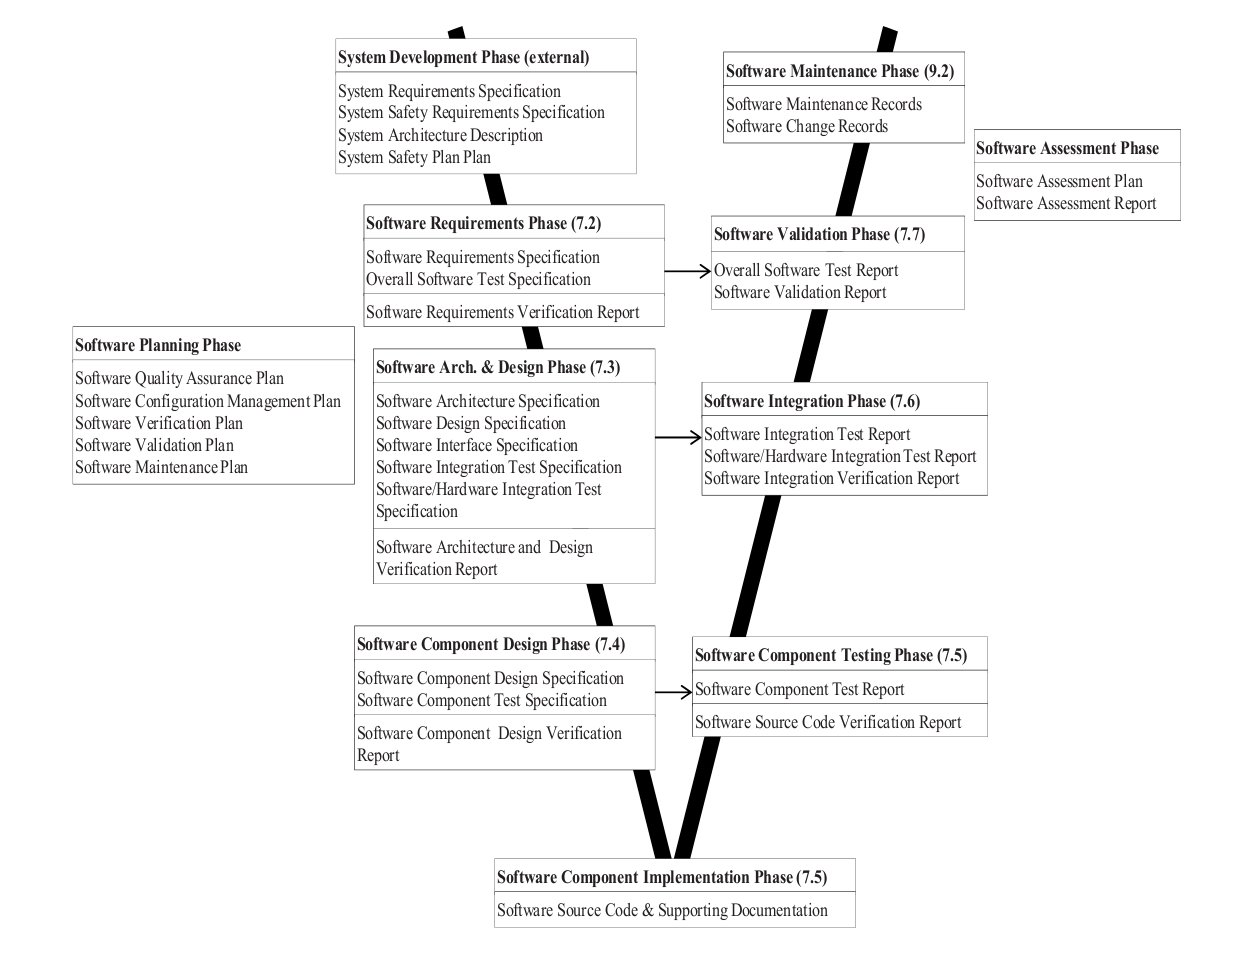
\includegraphics[width=\textwidth]{V-Model}
  \caption{General Development Lifecycle~\cite{EN-50128}}
  \label{fig:develop-lifecycle-cenelec}
\end{figure}

The recommended SW development lifecycle model in CENELEC EN 50128 is the
V-model as shown in Figure~\ref{fig:develop-lifecycle-cenelec}. It consists of
the SW planning phase in the beginning, the SW assessment phase at the end and
the following development phases:

\begin{itemize}
\item System Development Phase
\item SW Development Phases
  \begin{itemize}
  \item SW Requirements Phase
  \item SW Architecture and Design Phase
  \item SW Component Design Phase
  \item SW Component Implementation Phase
  \end{itemize}
\item SW Test / Validation Phases
  \begin{itemize}
  \item SW Validation Phase
  \item SW Integration Phase
  \item SW Component Testing Phase
  \end{itemize}
\end{itemize}

Each of the SW development phases shall have an appropriate test / validation
counterpart, as illustrated in the V form of the lifecycle. The implementation
of this generic process shall in particular focus on the usage of formal
methods. This has the following primary objectives:

\begin{itemize}
\item Increase the quality of the product wrt. safety
\item Allow for early discovery of errors in the  specifications
\item Replacement of manual steps by automatic transformations with proven
  properties
\end{itemize}

For each of the development phases of the lifecycle model of the standard, we
will propose how formal methods should be applied for openETCS.

\subsection{System Development Phase}
\label{sec:syst-devel-phase}

\paragraph{Objectives:}
\label{sec:sys-dev-objective}
In the system development phase, the requirements of the system and its safety
requirements shall be formalized. There shall also be a description of the
overall system architecture, preferably in a suitable graphical modeling
language\footnote{\eg, SysML~\cite{SysMLSpec}}. To exploit this model the most,
a model-driven engineering approach shall be used, where the model shall be
further refined in the later phases, \eg, with a detailed behavioral model. It
shall serve for documentation purposes, provide requirements traceability and
parts of it will be refined up to the algorithmic model of the executable code.

\paragraph{Formal Methods:}
\label{sec:sys-dev-formal-methods}
The system requirements and the safety requirements shall be formalized in
appropriate formal specification languages. In the system development phase,
this will be a rather high level modeling of the properties. Where possible, the
requirements will be referring the system architecture model to facilitate
traceability in later phases. The properties will be refined together with the
model in later phases.

The formalization of the requirements allows for the verification of
consistency, \eg, non-contradiction of the properties. This ensures the internal
consistency of the system requirements and the safety requirements, as well as
the consistency of the system requirements wrt. safety requirements. Tracing of
these requirements to the specification will ensure their completeness.

Any discovered deviation from the specification shall be documented. The
documented deviation shall then be used to enhance the informal system
specification, either by removing inconsistencies from or resolving ambiguities
in the informal requirements specification.

\paragraph{Documents:}
\label{sec:sys-dev-documents}
The documents to produce in this phase are the system safety plan, the system
requirements specification, the system architecture description and the software
/ hardware interface definition. The system safety plan explains the overall
approach to ensure safety in the developed system. The system requirements
specification describes all requirements of the system in a formal
language. This phase shall also produce the system architecture specification
and SW / HW interface definition which specify how the SW and the HW interact
and the location of the boundary between the two.


\paragraph{Detailed Description:}
\label{sec:sys-dev-deta-descr}
Figure~\ref{fig:detailed-sys-dev-phase} describes an iteration in this phase in
more detail.

\begin{figure}[ht]
  \centering
  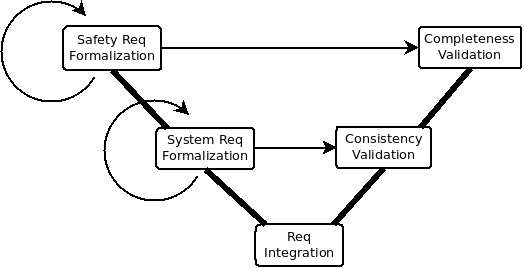
\includegraphics[width=.5\textwidth]{System-Dev-Phase-Details}
  \caption{Sub Process in System Development Phase}
  \label{fig:detailed-sys-dev-phase}
\end{figure}

The first phase is the formalization of the safety requirements, this it
iterated until internal consistency is ensured. The next phase is the
formalization of the system requirements, analogously with an iteration to
ensure their consistency.

Both sets of requirements are combined in the requirement integration
phase. They shall be transformed into a common formal specification format if
necessary. The consistency of the combination is verified in the next phase and
finally the completeness of the requirement wrt. informal specification. Any
deviation from the consistency of the combined requirements or from the
completeness shall be documented and the phases reiterated until consistency and
completeness is achieved.


\subsection{SW Development Phase}
\label{sec:sw-development-phase}

\subsubsection{SW Requirements Phase}
\label{sec:sw-requ-phase}

\paragraph{Objectives:}
\label{sec:sw-req-objective}
In this phase, the SW requirements shall be described and formalized based on
the results of the preceding phase, \ie, the formal system requirements, the
formal safety requirements and the system architecture specification. The part
of the system model concerning the software will further be refined, ensuring
traceability of the software requirements. All existing constraints of the
constraints between HW and SW will be taken into account.

\paragraph{Formal Methods:}
\label{sec:sw-req-formal-methods}
The SW requirements shall be formalized in an appropriate formal specification
language. In the software requirements phase, this will be a rather high level
modeling of the properties, similar to the system requirements
specification. The part of the system architecture model which concerns the SW
implementation of the system shall be refined and the SW requirements shall be
referenced in it.

The formalization of the SW requirements shall be used to ensure their internal
consistency and their correctness and completeness wrt. the system requirements
specification and the safety requirements specification.

The SW requirements specification shall list all functions which will be
performed by the SW, identifying each safety related function. For each
function, it will specify all required input signals and admissible values, the
expected output and the test criteria including performance and quality aspects.

A formal model of the behavior of the programmable electronic hardware shall be
established. This model shall in particular describe the modes, the transitions
between the modes and shall include the failure behavior. The correctness of
this model according to the relevant parts of the safety specification shall be
verified with appropriate formal verification techniques. Any deviation of the
behavior shall be documented and fixed in a succeeding iteration. The documented
deviations shall be used as test cases in the SW test specification.


\paragraph{Documents:}
\label{sec:sw-req-documents}
The documents to produce in this phase are the SW testing
specification and the SW requirements verification report. The SW testing
specification (see 6.2, A.5) will provide the detailed approach to test the
developed SW, concertizing the approach in the SW testing plan. This shall
provide the information where formal verification will be used, in particular
where formal techniques like proofs will replace testing of the developed SW.
The SW requirements verification report will document the results of the
verification of the SW requirements specification wrt. the criteria specified in
7.2.4.22 of the standard.

\paragraph{Responsible:}
\label{sec:sw-req-responsible}
RQM

\paragraph{Detailed Description:}
\label{sec:sw-req-deta-descr}
Figure~\ref{fig:detailed-sw-dev-phase} shows the sub-phases of the SW
requirements phase.

\begin{figure}[ht]
  \centering
  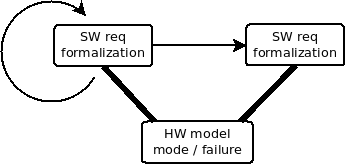
\includegraphics[width=.35\textwidth]{SW-Req-Phase-Details}
  \caption{Sub Process in SW Development Phase}
  \label{fig:detailed-sw-dev-phase}
\end{figure}

The first phase consists of the description and formalization of the SW
requirements. The system architecture model from the preceding phase shall be
extended with a model of the SW. All SW requirements shall be referenced in that
model. The internal consistency of the SW requirements shall be verified with an
appropriate formal verification tool, any inconsistency shall be
documented. This shall be iterated until consistency of the SW requirements is
achieved.

In the next phase a formal behavioral model of the programmable electronic HW is
produced which includes in particular the desired behavior in case of
failures.

The SW requirements together with the HW model are combined in an appropriate
formal specification  and the consistency and correctness wrt. the system
requirements and the safety requirements shall be verified formally. The
deviations shall be documented. They shall be fixed in the next in-phase
iteration.



\subsubsection{SW Architecture and Design Phase}
\label{sec:sw-arch-design}


\subsubsection{Objectives:}
\label{sec:sw-arch-objectives}
In this phase a SW architecture shall be developed which allows to meet the SW
requirements and the necessary safety requirements without introducing
unnecessary complexity. In this phase there shall also be an evaluation of the
HW / SW interaction, its influence on the safety aspects of the system and the
valuation of the usage of already existing SW. It shall also ensure the
testability and the appropriateness for formal proofs of the resulting SW, in
particular by minimizing the complexity and the size of the safety relevant
parts.

\subsubsection{Formal Methods:}
\label{sec:sw-arch-formal-methods}
This phase shall develop a formal description of all SW interfaces; those
between different SW components and between newly developed SW and already
existing SW. This shall include pre- and postconditions, boundary values for all
parameters, the behavior if those conditions are not met, memory allocation
etc. (for a full list see 7.3.4.19) ($\rightarrow$ Software interface
specification).

The architecture and design phase shall develop the description of the SW
components which will be developed. The exiting formal SW model will therefore
be refined to the SW components of the architecture. The SW requirements and
safety requirements will be refined to requirements for the components and the
necessary SIL for each component shall be identified. It shall be formally
verified, that the SW requirements for the components are consistent wrt. global
SW requirements and the safety requirements. ($\rightarrow$ Software design
specification).

For the later integration of the software, a formal behavior model of the system
into which the SW will be integrated shall be developed. To achieve this, the
behavioral model of the earlier phases shall be refined and it shall be verified
that the SW behaves as expected wrt. system into which it will be
integrated. Any deviation of this behavior shall be documented and integrated
into the software integration test specification as test-case.

\subsubsection{Documents:}
\label{sec:sw-arch-documents}
In this phase the following documents shall be produced: the
specifications for the SW architecture, the SW design and the SW interface,
there shall also be the specification for the SW integration test and for the SW
/ HW integration test. Finally the SW architecture and design verification
report will document whether this phase has been finished in accordance with
the standard.

\subsubsection{Responsible:}
\label{sec:sw-arch-responsible}
DES, VER, INT

\subsubsection{Detailed Description:}
\label{sec:sw-arch-deta-descr}
The details of the sub-process of the SW architecture and design phase is shown
in Figure~\ref{fig:detailed-sw-arch-phase}.

\begin{figure}[ht]
  \centering
  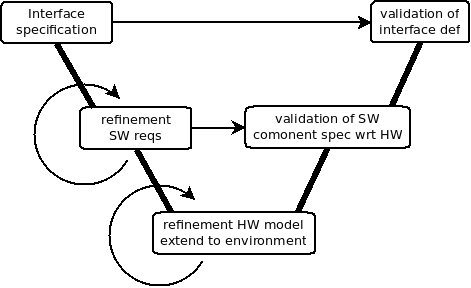
\includegraphics[width=.5\textwidth]{SW-Arch-Phase-Details}
  \caption{Sub Process in SW Architecture and Design Phase}
  \label{fig:detailed-sw-arch-phase}
\end{figure}

In the first phase the interfaces of the SW to other SW and to HW shall be
formally defined in an appropriate specification language. In particular the
necessary pre- and postconditions, used parameters and their boundaries shall be
described in a formal way~\footnote{\eg, in ACSL~\cite{baudin09acsl} the
  annotation language used by Frama-C (\url{http://frama-c.com})}

The next step is to refine the SW architecture to components. The SW
requirements specification shall be refined to these components. It shall be
formally verified that the requirements of the components are internally
consistent and that they are correct wrt. SW requirements specification. Any
found deviation shall be documented and the sub-phase shall be iterated until
consistency and correctness is achieved.

The model of the programmable HW shall be further refined and be extended with a
formal description of the system into which the SW will be integrated. This
model shall be verified wrt. safety requirements, any deviation shall be
documented and fixed for a later iteration of this sub-phase.

The consistency of the SW component requirements specification wrt. the HW
behavioral model shall be verified, as well as the consistency of the interface
definition wrt. SW components and the HW parts of the system. Deviations shall
be recorded and the sub-phase shall be iterated until consistency is reached.


\subsubsection{Software Component Design Phase}
\label{sec:softw-comp-design}

\paragraph{Objectives:}
\label{sec:sw-comp-objectives}
This phase shall develop a low level specification for each of
the SW components which is correct wrt. requirements of the SW design
specification and of the SW component design specification.

\paragraph{Formal Methods:}
\label{sec:sw-comp-formal-methods}
This phase shall make the most elaborate use of formal methods in the
development process. The formal model describing the system shall be further
refined up to the algorithmic description on the SW component level.

Together with the specification of the various interfaces, the pre- and
postconditions, the algorithms to use and the description of the data
structures, a detailed formal model of the behavior shall be produced for each
SW component. This model shall be expressed in an appropriate formalism for
which an appropriate tool exists such that the SW and safety requirements can be
proven and the actual source code can be generated automatically.

\paragraph{Documents:}
\label{sec:sw-comp-documents}
In this phase, the produced document will be the formal refinement and
verification report created by the formal proofs. This shall describe the proof
steps, the refinements and the necessary lemmas to prove the properties and the
refinements. The document shall also include the necessary justifications to
replace the manual step of SW component implementation and SW component unit
tests.

\paragraph{Responsible:}
\label{sec:sw-comp-responsible}
DES, VER

\paragraph{Detailed Description:}
\label{sec:sw-comp-deta-descr}
This phase shall replace the manual steps component implementation and component
testing with unit-tests which are present in the original development
lifecycle. The formal proofs will ensure correctness of the generated code
wrt. specification, therefore making testing superfluous. The outline of this is
shown in Figure~\ref{fig:proof-code-generation}, where the green arrow marks the
proposed ``shortcut''. According to the standard, such an approach and the
applied tools must be appropriate according to 6.7.4.4.

\begin{figure}[ht]
  \centering
  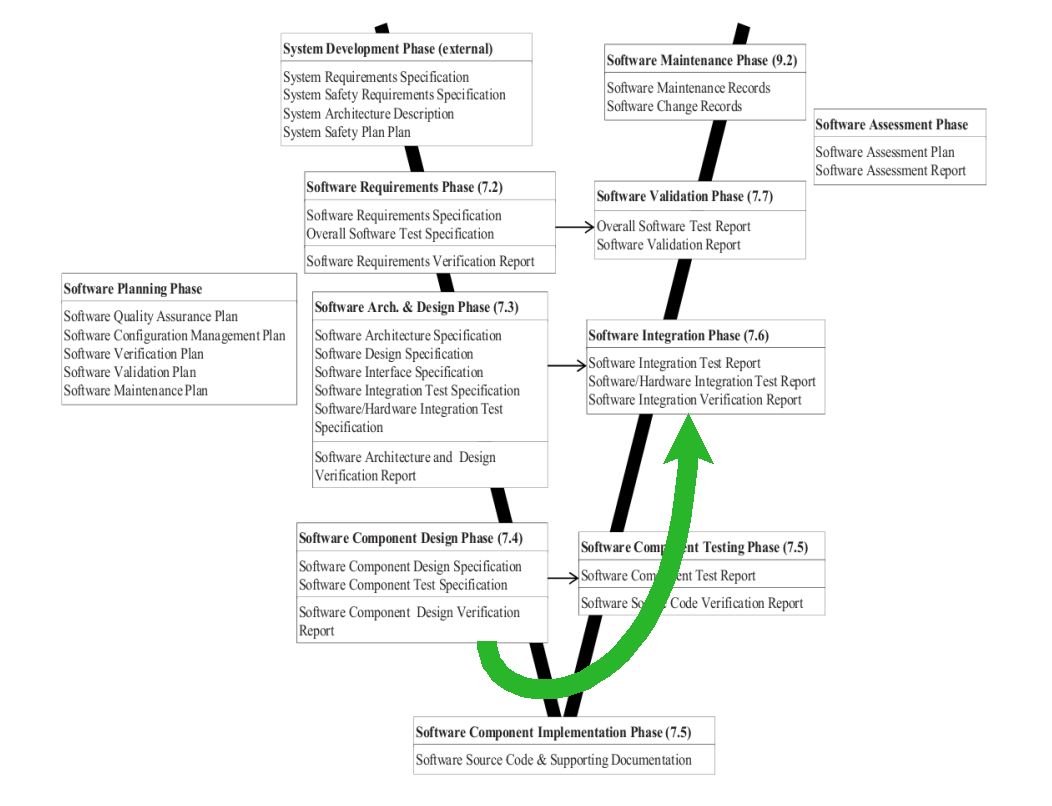
\includegraphics[width=\textwidth]{V-Model-abk}
  \caption{Formal Proof and Automatic Code Generation in V-Model}
  \label{fig:proof-code-generation}
\end{figure}

The sub process in this phase is shown in
Figure~\ref{fig:detailed-sw-comp-phase}.

\begin{figure}[ht]
  \centering
  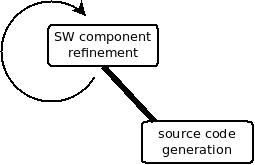
\includegraphics[width=.3\textwidth]{SW-Comp-Phase-Details}
  \caption{Sub Process in SW Component Design Phase}
  \label{fig:detailed-sw-comp-phase}
\end{figure}

The SW component refinement phase shall verify the correctness of the refinement
wrt. the SW component requirements specification. This sub-phase shall be
iterated until the specification of the behavior of each SW component is
detailed enough to be eligible to automatic code generation. A suitable
formalism for this approach shall be a formal framework which supports formal
proofs of properties, supports iterative refinement, supports refinement proofs
and is suitable wrt. criteria of the standard\footnote{\eg, the Event-B method
  as integrated int the Rodin tool~\cite{Abrial:Rodin}
  (\url{http://www.event-b.org/})}. Finally the source code shall be generated
from the formal behavior specification.

Although automatically generated, the source code shall contain annotations for
the pre- and postconditions and other properties, \eg, loop invariants. The
generated code shall also adhere to the coding standards of as defined in the SW
design specification. This will ensure that the generated code is human readable
and facilitate its potential re-use in other projects.


\subsubsection{Software Component Implementation Phase}
\label{sec:softw-comp-impl}

Shall be replaced by automatic code generation from formal models using
refinement techniques.

\subsubsection{Software Component Testing Phase}
\label{sec:softw-comp-test}

Shall be replaced by giving formal proofs of the generated code and showing the
adherence to all SW and safety requirements by the formal model.

\subsubsection{Software Integration Phase}
\label{sec:softw-integr-phase}

\paragraph{Objectives:}
\label{sec:sw-int-objectives}
This phase shall demonstrate the correct functioning of the combination of the
developed SW components, in particular in their target HW environment. The
necessary tests for this phase are specified in the SW / HW integration test
specification and SW integration test specification.

\paragraph{Formal Methods:}
\label{sec:sw-int-formal-methods}
Any deviation which is found in this phase shall be documented. The results of
this phase shall be used to refine the formal models if necessary, in particular
the formal models of the HW.

\paragraph{Documents:}
\label{sec:sw-int-documents}
The SW integration test report shall document the results from the integration
of the SW, the SW / HW integration report the results from the integration of
the developed SW on the target HW. Both shall include the test cases, their
respective results and document all details of the configuration for the
tests. The SW integration verification report shall document whether the test
reports have been written according to their respective specifications and
adhere to the relevant parts of the standard for test reports.

\paragraph{Responsible:}
\label{sec:sw-int-responsible}
INT, VER

\subsubsection{Overall Testing / Final Validation}
\label{sec:overall-testing-}

\paragraph{Objectives:}
\label{sec:sw-test-objectives}
The objective of this phase is to validate the adequacy of the developed SW and
its integration wrt. system requirements specification, the functional
properties and the safety related properties of the system according to the
SIL. In this phase the overall fitness for purpose of the system will be
evaluated.

\paragraph{Formal Methods:}
\label{sec:sw-test-formal-methods}
This phase is executed by the VAL who will validate the developed system. In
particular, he will analyze whether the chosen combination of techniques are
appropriate wrt. standard, \eg, the use of formal proofs in
phase~\ref{sec:softw-comp-design} to replace phases~\ref{sec:softw-comp-impl}
and~\ref{sec:softw-comp-test}.

\paragraph{Documents:}
\label{sec:sw-test-documents}
The VAL will produce the overall SW test report in which the VAL will document
the results of additional tests he specified and executes himself or lets TST
execute them. The VAL will also produce a SW validation report which shall
document the results of the SW validation plan. The VAL will also produce a
release note which shall document any restriction of the usage of the developed
software.

\paragraph{Responsible:}
\label{sec:sw-test-responsible}
VAL


\subsection{Conclusion}
\label{sec:conclusion-fm-process}

The focus on the application of formal methods in the proposed development
process will lead to an increased quality and reduced development cost. In
particular, formal methods will support the early detection and elimination of
design flaws through rigorous formal analysis in the in-phase iterations. Early
error detection can greatly reduce the cost, in particular for safety relevant
SW development, by avoiding to have to redo several test and validation steps.

The envisioned automatic code generation by refinement will formally proof the
correctness of the resulting SW wrt. its specification. This will increase the
quality of the resulting code, as well as eliminate the need for verification of
adherence to coding standards and for unit tests of SW components.

The proposed model-driven approach with model refinement will facilitate the
production of documentation and traceability of the requirements according to
the requirements of the standard. An important aspect to implement this approach
is the application of an appropriate supporting tool chain, in particular with
exchangeable file formats for the respective models.

Figure~\ref{fig:overview-models-process} present an overview of the generated
models and their relation. The solid arrows in both direction indicate a formal
verification of consistency (and correctness), the dashed arrows in one
direction indicate a refinement. The pointed line indicate the different phases
of the process.

\begin{figure}[ht]
  \centering
  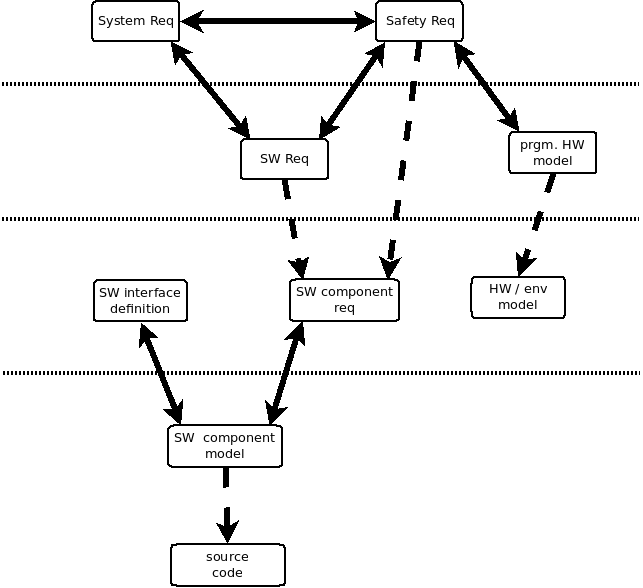
\includegraphics[width=.5\textwidth]{ProcessBild}
  \caption{Overview of Formal Models Generated in Process}
  \label{fig:overview-models-process}
\end{figure}

A prime candidate for this is the Eclipse platform, which is well extensible and
provides support for XML based file exchange formats. It is also the basis for
model-based development tools like
TopCASEd\footnote{\url{http://www.topcased.org/}}, provides integration for
requirements engineering tools like
ProR\footnote{\url{http://www.eclipse.org/rmf/pror/}} and forms the basis for
the formal proof tool Rodin.


%%% Local Variables:
%%% mode: latex
%%% TeX-master: "wp-2.2"
%%% End:
